\documentclass[10pt]{article}
\setlength{\parskip}{0.25\baselineskip}
\usepackage[margin=1in]{geometry} 
\usepackage{amsmath,amsthm,amssymb, graphicx, multicol, array}
\usepackage[font=small,labelfont=bf]{caption}
\usepackage{float}
\usepackage{bbm}

\newcommand{\supp}{{\text{supp}}} 
\newcommand{\bv}{{\text{BV}}}
\newcommand{\ac}{{\text{AC}}}
\newcommand{\vol}{{\text{Vol}}}

\newenvironment{problem}[2][]{\begin{trivlist}
\item[\hskip \labelsep {\bfseries #1}\hskip \labelsep {\bfseries #2.}]}{\end{trivlist}}

\begin{document}
 
\title{Homework \#7}
\author{Eric Tao\\
Math 123: Homework \#7}
\maketitle

\begin{problem}{Question 1}

Consider the cube $C_r^D = [-r/2, r/2]^D \subset \mathbb{R}^D$ in $D$ dimensions. Let $\vol_D(A)$ denote the volume of a set $A$ in $\mathbb{R}^D$, that is:

$$ \vol_D(A) = \int_A dx_1...dx_D$$

(a) Prove using integration, that $\vol_D(C_r^D) = r^D$.

(b) For an $\epsilon > 0$, define $A_{\epsilon,r}^D = \{ x \in C_r^D : x \not \in C_{r - \epsilon}^D \}$. Compute

$$ \frac{\vol_D(A_{\epsilon, r}^D)}{\vol_D( C_r^D)}$$

(c) Using (b), argue that most of the volume for a high-dimensional cube is near the boundary. Can you make this precise?

\end{problem}

\begin{proof}[Solution]

(a)

Without too much difficulty, we see that:

$$\int_{C_r^D} dx_1...dx_D = \underbrace{ \idotsint_{-r/2}^{r/2}}_{D \text{ times}} dx_1 \cdots dx_D = \left( \frac{r}{2} - \frac{-r}{2} \right)^D = r^D$$

(b)(c)

Similarly, here, we compute $\vol_D(A_{\epsilon, r}^D) = \vol_D( C_r^D) - \vol_D( C_{r-\epsilon}^D)$. But, from part (a), we have that:

$$\vol_D(A_{\epsilon, r}^D) = \vol_D( C_r^D) - \vol_D( C_{r-\epsilon}^D) =r^D - (r - \epsilon)^D $$

Then, we have that:

$$ \frac{\vol_D(A_{\epsilon, r}^D)}{\vol_D( C_r^D)} = \frac{r^D - (r - \epsilon)^D}{r^D}= 1 - \left(1 - \frac{\epsilon}{r}\right)^D$$

If we do a second order approximation, assuming $\frac{\epsilon}{r}$ is small, then we can say:

$$  \left(1 - \frac{\epsilon}{r}\right)^D \approx 1 - \frac{D \epsilon}{r}+ \frac{D(D-1)}{2} \frac{\epsilon^2}{r^2} $$

Then we have that:

$$\frac{\vol_D(A_{\epsilon, r}^D)}{\vol_D( C_r^D)} \approx \frac{D \epsilon}{r} - \frac{D(D-1)}{2} \frac{\epsilon^2}{r^2}$$

Setting this equal to one half, we can solve for $z = \frac{\epsilon}{r}$:

$$ 2Dz - D(D-1) z^2 = 1 \implies D(D-1) z^2 - 2Dz + 1 = 0 \implies z = \frac{2D \pm \sqrt{4D^2 - 4(D^2 - D)}}{2D(D-1)} = \frac{D \pm \sqrt{D}}{D(D-1)}$$

We see that in the limiting case as $D \to \infty$, the denominator grows as $D^2$, compared to $D$ for the numerator, so $\epsilon/r \to 0$ as $D$ is large. We can conclude that for arbitrarily large dimensions, the proportion of the cube tends to lie nearer to the boundary, in terms of percentage of the side of the cube.


\end{proof}

\begin{problem}{Question 2}

Fix some $w \in \mathbb{R}^{D \times 1}$.

(a) Show that $\{ x \in \mathbb{R}^{D \times 1} : w^T x = 0 \}$ is a $(D-1)$-dimensional linear subspace of $\mathbb{R}^D$, if $w \not = 0$.

(b) Fix some $b \in \mathbb{R}$. Is the set $\{ x \in \mathbb{R}^{D \times 1} : w^T x = b \}$ a $(D-1)$-dimensional linear subspace of $\mathbb{R}^D$? Prove or show a counterexample.


\end{problem}

\begin{proof}[Solution]

(a)

Viewing $w^T$ as a matrix, we see that this has one row and $D$ columns. Thus, it is already in reduced row echelon form. Thus, there are $D-1$ columns that do not have pivots, and thus the nullspace has dimension $D-1$, and is a linear subspace. But that is exactly $\{ x \in \mathbb{R}^{D \times 1} : w^T x = 0 \}$.

(b)

Actually, we see that  $\{ x \in \mathbb{R}^{D \times 1} : w^T x = b \}$ is trivially not a subspace, since the zero vector is never in this set. However, due to linearity, we may identify it as a copy of $\mathbb{R}^{D-1}$. In particular, we may view it as a coset of the nullspace: Take any solution $x_0$ to $w^Tx = b$ which must exist, since we may always identify some non-0 component of $w$, say, $w_j$, and choose the vector 0 everywhere except $\frac{b}{w_j}$ in the $j$-th coordinate, and then identify the solution set as:

$$\{  x_0 + y : w^T y = 0 \}$$

By part (a), the set of basis vectors has $D-1$ vectors, however, it does not constitute a linear subspace.



\end{proof}

\begin{problem}{Question 3}

Using the dataset "kNN\_ClassifierSyntheticData.mat", randomly select 100 different testing points in the dataset, and run a kNN-classifier for kNN $= \{ 1,10,50,100,500,900 \}$ using the remaining points as training points. How does performance change with the change in kNN?

\end{problem}

\begin{proof}[Solution]

Running a classifier, we find the following accuracy measures, where we define accuracy as the number of labels learned that coincide with the labels predicted, divided by the number of testing points in the data set.

If we graph the accuracy, this is what we find:

\begin{center}
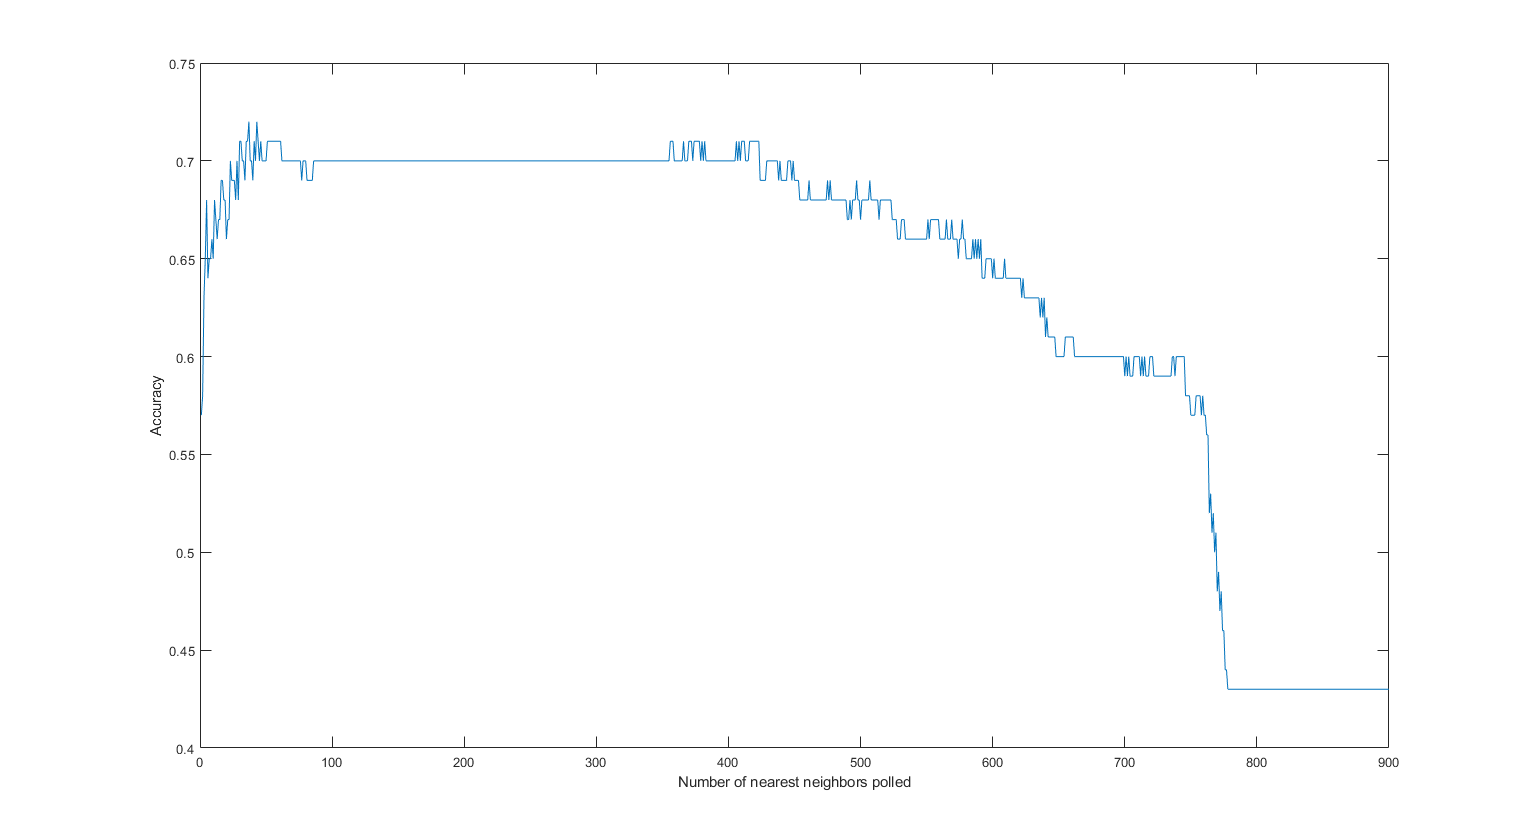
\includegraphics[width=\linewidth]{knn_synthetic_data_accuracy}
\captionof{figure}{kNN Accuracy Synthetic Data}
\end{center}

In particular, we find the following values:

\begin{center}
\begin{tabular}{|| c| c||}
\hline
kNN & Accuracy \\

\hline \hline
1 & 57\% \\ \hline
10 & 65\% \\ \hline
50 & 70\% \\ \hline
100 & 70\% \\ \hline
500 & 67\% \\ \hline
900 &  43\% \\ \hline
\end{tabular}
\end{center}

We see that at extreme values of $kNN$, that is, nearly all of the training data or very few neighbors, close to 1 or 900, the accuracy tends to be low. The low end tends to be low accuracy because of potentially not polling enough data points, and the high end is a result of overtuning onto the training set. Instead, accuracy is best somewhere in the middle, which graphically looks to be in the $kNN \approx 50$ range, but is fairly stable up until $kNN \approx 450$.


\end{proof}

\begin{problem}{Question 4}

Using the Salina A dataset, randomly select $100$ different testing points in the dataset, and run a kNN-classifier for kNN $= \{ 1,10,50,100,500,900 \}$ using the remaining points as training points. How does performance change with the change in kNN?


\end{problem}

\begin{proof}[Solution]

Here, we do something very similar, though instead of using the synthetic data that was pregenerated, we will be using the Salinas A groundtruth as our labels. In this case then, we will have 7 distinct labels:

\begin{center}
\begin{tabular}{|| c| c||}
\hline
Label & Ground Truth \\

\hline \hline
0 & Misc \\ \hline
1 & Brocoli\_green\_weeds\_1 \\ \hline
10 & Corn\_senesced\_green\_weeds \\ \hline
11 & Lettuce\_romaine\_4wk \\ \hline
12 & Lettuce\_romaine\_5wk \\ \hline
13 &  Lettuce\_romaine\_6wk \\ \hline
14 & Lettuce\_romaine\_7wk \\ \hline
\end{tabular}
\end{center}

Plotting accuracy again, we see that:

\begin{center}
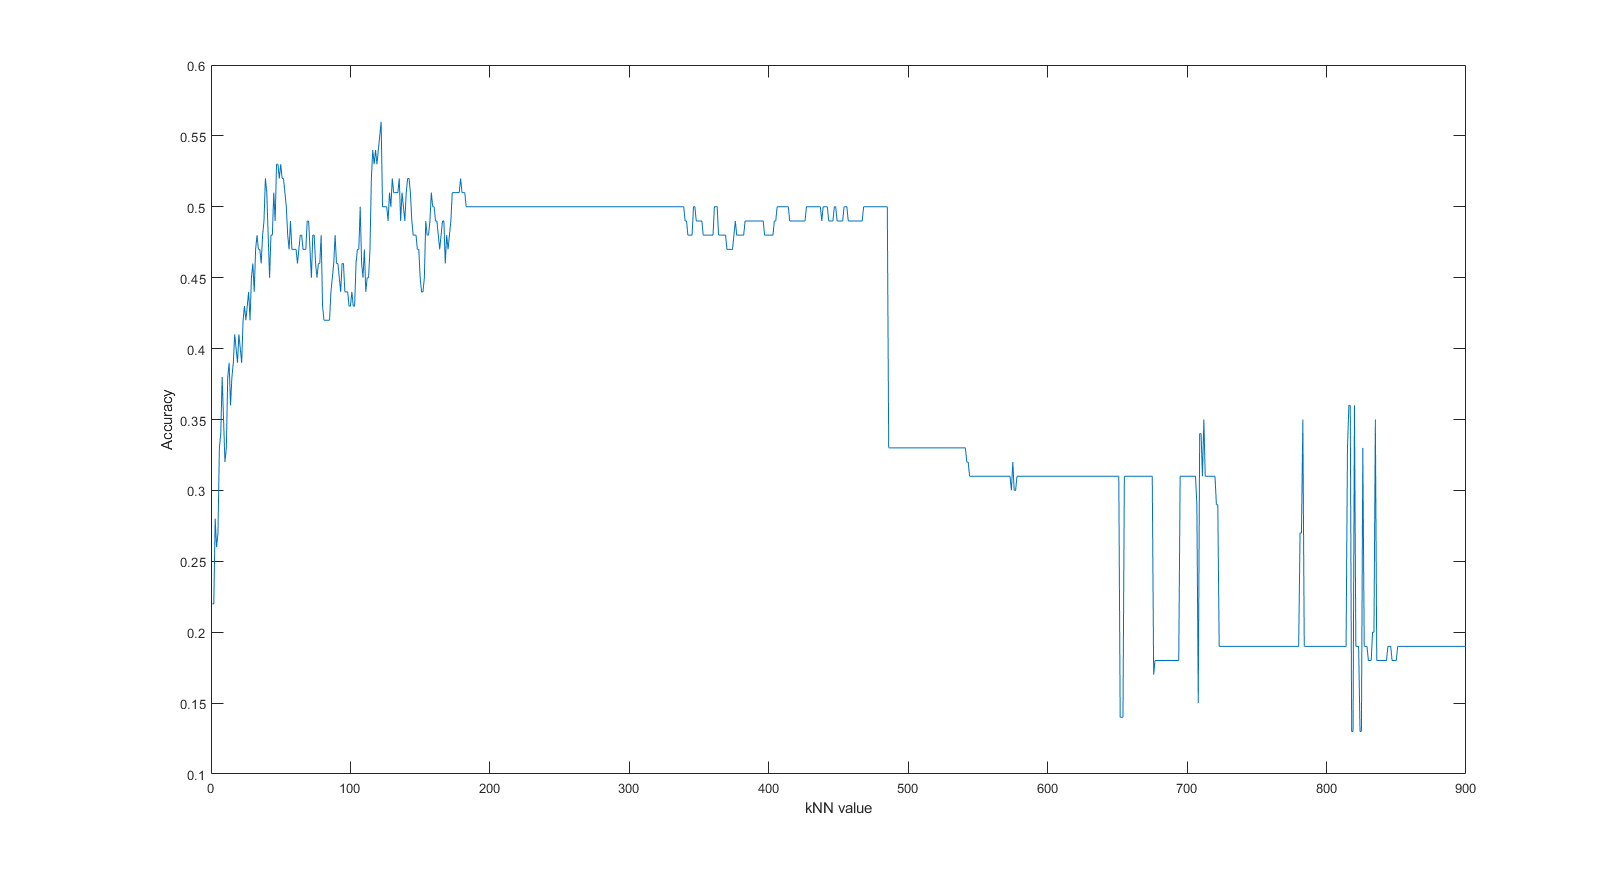
\includegraphics[width=\linewidth]{knn_salinas_accuracy}
\captionof{figure}{kNN Accuracy Salinas A}
\end{center}

Similar to the synthetic data case, we see here that at very low values of $kNN$, in our case, visually, around $0-50$, accuracy increases. However, as $kNN$ becomes very large, the model overtunes to the training data, and loses accuracy, here past $kNN = 500$. Visually, accuracy looks to be best at the 120 range, but is very stable in the 200-475 range or so.

In particular, the exact values are as follows:

\begin{center}
\begin{tabular}{|| c| c||}
\hline
kNN & Accuracy \\

\hline \hline
1 & 22\% \\ \hline
10 & 32\% \\ \hline
50 & 53\% \\ \hline
100 & 43\% \\ \hline
500 & 33\% \\ \hline
900 &  19\% \\ \hline
\end{tabular}
\end{center}

\end{proof}


\end{document}